% TeX root=../main.tex

\chapter{Sintaxe}

\section{Concordância}

\section{Uso dos casos}

\section{Comparação}

\section{Advérbios}

\section{Posposições}

\section{Pronomes}

\section{Ordem de palavras}

\section{Interrogações}

\section{Coordenação}

\section{Subordinação}

\paragraph{Causais}

\paragraph{Condicionais}

\paragraph{Concessivas}

\paragraph{Consecutivas}

\paragraph{Relativas}

\paragraph{Temporais}
\ldots{}

\clearpage
\chapter{Leitura: BOHÇA}


A inscrição (\autoref{fig:bohça}) é conhecida desde 1901, tendo sido encontrada
em uma colina do vilarejo de Bohça (Bozca ou Bahçeköy),
provavelmente no contexto original e está atualmente locada no Kayseri
Arkeoloji Müzesi (no.\ 6).
O governante Kurtis filho de Ashwisis talvez possa ser identificado com o
mesmo governante mencionado por Sargão II por Kurti de Atunna entre 718--713
\textsc{aec}, e o estilo da inscrição corresponde ao esperado para este
período.
A associação, no entanto, depende da localização de Atunna.
Bohça está no meio da região conhecida das fontes
neo-assírias pelo nome de Tabal que, na idade do ferro, era composta por
diversas pequenas cidades-estado.

\begin{center}
	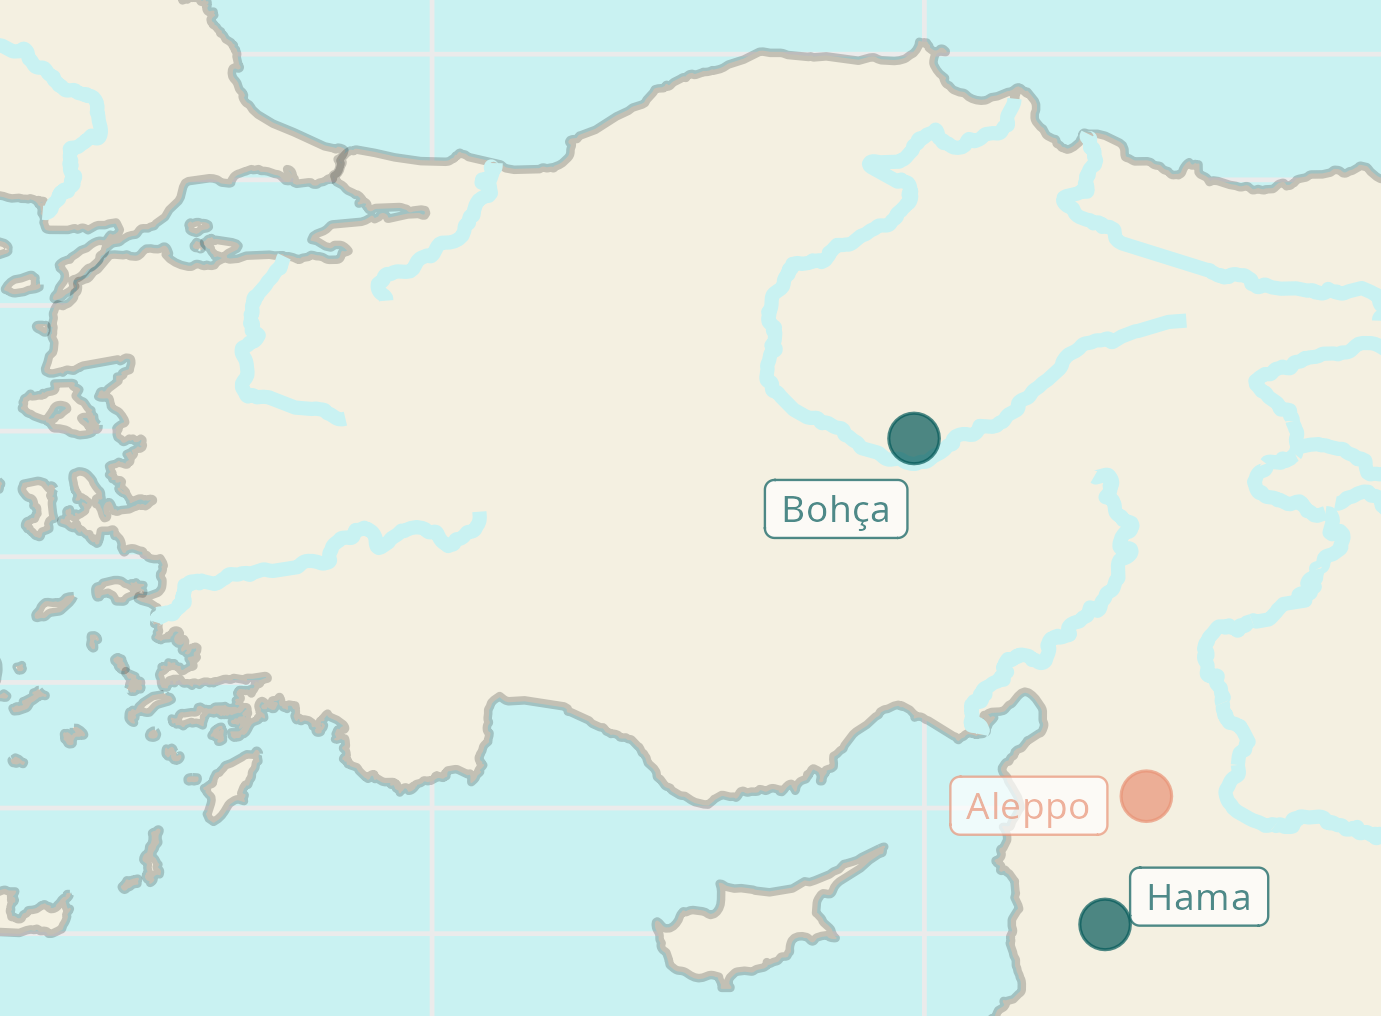
\includegraphics[width=0.65\textwidth]{../../../Mídia/Map03.png}
\end{center}


\begin{figure}[h]
	\centering
	\begin{subfigure}{0.49\textwidth}
		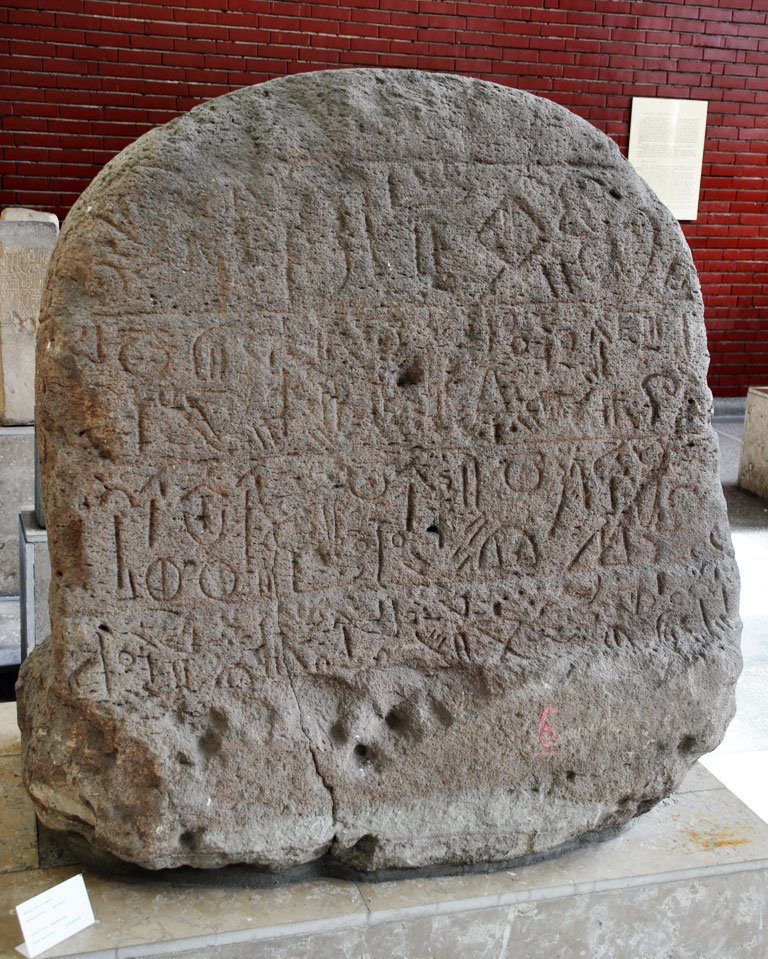
\includegraphics[width=0.9\textwidth]{../../../Mídia/bahce08.jpg}
	\end{subfigure}
	\hfill
	\begin{subfigure}{0.49\textwidth}
		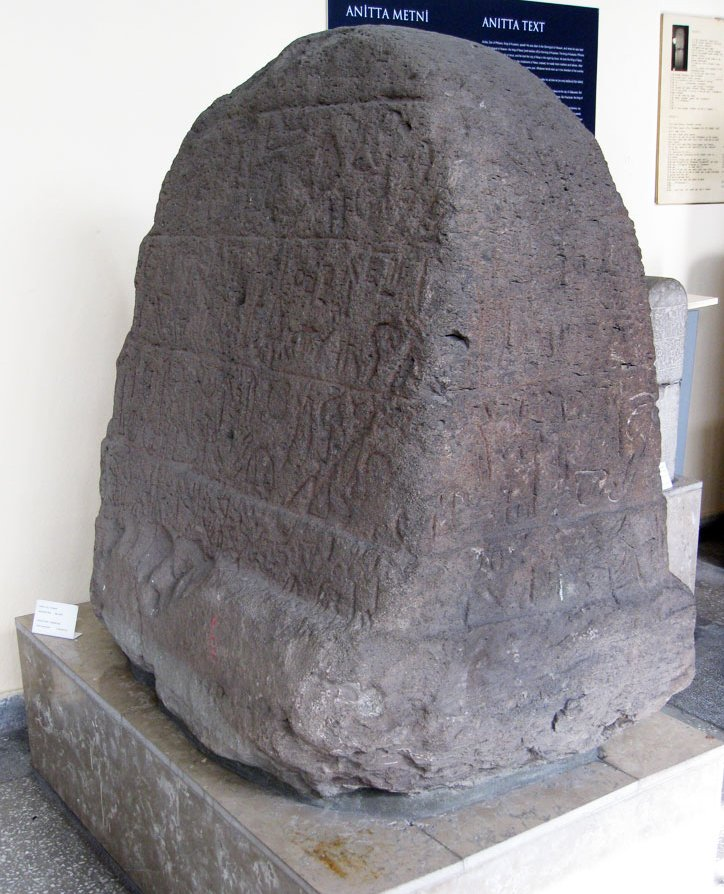
\includegraphics[width=0.9\textwidth]{../../../Mídia/bahce10.jpg}
	\end{subfigure}
	\caption[BOHÇA]{Inscrição BOHÇA. Dimensões da inscrição:
		1.26\times0.63m.
		Imagens de Cüneyt Süer, 2011,
		disponíveis em
		\href{https://www.hittitemonuments.com/bahcekoy/}{Hittite Monuments}.
		Edição e traçado em~\citeabbrev*{CHLI11}, pp.\ 478ff.\ e \emph{plate}
		265.
	}\label{fig:bohça}
\end{figure}

\clearpage

\begin{center}
	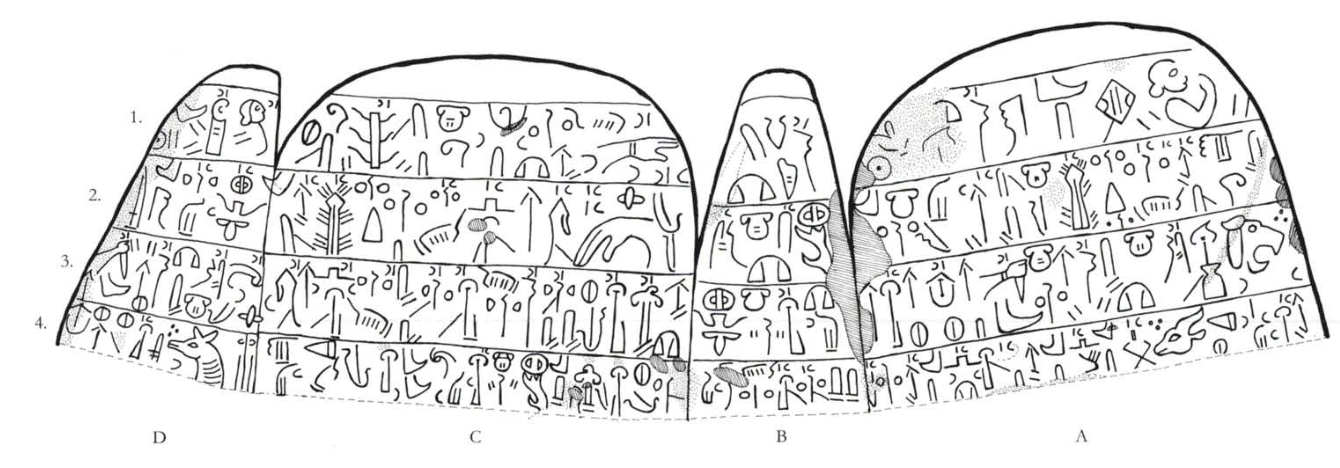
\includegraphics[width=\textheight,angle=90]{../../../Mídia/bohça.png}
\end{center}



\clearpage
\begin{parnumbersa}[]
	\raggedright%

	\Large \luwiantrans{EGO-mi}\hspace{5pt}
	[\luwmasc]\luwiantrans{ku-ra-ti-i-sá}\hspace{5pt}
	\luwmasc\luwiantrans{á-[sa-hwi-si]-sa4}\hspace{5pt}
	\luwmasc\luwiantrans{HEROS-li-i-sa}\hspace{5pt}
	\luwmasc\luwiantrans{<FILIUS>-ni-mu-wi-za-sa}\hspace{5pt}
	\luwiantrans{<OCCIDENS>-i-pa-ma-i+ri-i}\hspace{5pt}
	\luwmasc\luwiantrans{ORIENS-mi-ma-i+ri-ha}\hspace{5pt}
	\luwmasc\luwiantrans{PRAE}\hspace{5pt}
	\luwmasc\luwiantrans{AUDIREMI-ti-mi-sa4}\hspace{5pt}
	[\luwmasc]\luwiantrans{REX-ti-sá}\hspace{5pt}

	\Large \luwmasc\luwiantrans{wa-ta}\hspace{5pt}
	\luwmasc\luwiantrans{DEUS-TONITRUS-hu-ti}\hspace{5pt}
	\luwmasc\luwiantrans{za-i+ri}\hspace{5pt}
	\luwmasc\luwiantrans{BONUS-wa-su-wa-i}


	\Large \luwmasc\luwiantrans{wa-mu}\hspace{5pt}
	\luwmasc\luwiantrans{TERRA-REL-ra-zi}\hspace{5pt}
	\luwmasc\luwiantrans{SUPER-ra}\hspace{5pt}
	\luwmasc\luwiantrans{<CAPERE>-lu-na-'}\hspace{5pt}
	\luwmasc\luwiantrans{pi-pa-sa-i}\hspace{5pt}


	\Large \luwmasc\luwiantrans{DEUS-CERVUS3-ti-pa-wa-ta-'}\hspace{5pt}
	\luwmasc\luwiantrans{za-i+ri-ia-pa-a}\hspace{5pt}
	\luwmasc\luwiantrans{BONUS-wa-su-wa-i}


	\Large\luwmasc\luwiantrans{wa-mu}\hspace{5pt}
	\luwmasc\luwiantrans{za-ri+i}\hspace{5pt}
	\luwmasc\luwiantrans{sà-ma-ia}\hspace{5pt}
	\luwmasc\luwiantrans{<ANIMA-LEO>-hwi-sa5-ra}\hspace{5pt}
	\luwmasc\luwiantrans{pi-pa-sa-ia}


	\Large\luwmasc\luwiantrans{á-mi-zi-pa-wa}\hspace{5pt}
	\luwmasc\luwiantrans{tá-ti-zi-i}\hspace{5pt}
	\luwmasc\luwiantrans{AVUS-ha-zi-ha}\hspace{5pt}
	\luwmasc\luwiantrans{REL-zi}\hspace{5pt}
	[\luwmasc]\luwiantrans{sa-ta}\hspace{5pt}


	\Large\luwmasc\luwiantrans{REL-pa-wa}\hspace{5pt}
	\luwiantrans{DEUS-TONITRUS-hu-za-sa}\hspace{5pt}
	\luwmasc\luwiantrans{NEG2}\hspace{5pt}
	\luwmasc\luwiantrans{REL-ha-na}\hspace{5pt}
	\luwmasc\luwiantrans{wa-ra-ia-ia}\hspace{5pt}


	\Large\luwmasc\luwiantrans{á-mu=wa}\hspace{5pt}
	\luwmasc\luwiantrans{REL-ra}\hspace{5pt}
	\luwmasc\luwiantrans{wa-ra-ia-ia}\hspace{5pt}



\end{parnumbersa}

\vspace{10pt}
\hrule
\vspace{10pt}

\setcounter{parcount}{0}
\begin{parnumbersa}[]

	\raggedright%
	\itshape%

	\logo{EGO}-mi
	$[$\lmasc\textsuperscript{?}$]$ku+ra/i-ti-i-sá
	\lmasc{}á-[sa-hwi/a-si]-sa\textsubscript{4}
	\lmasc{}\logo{HEROS}-li-i-sa
	\lmasc{}\logo{``FILIUS''}-ni-mu-wa/i-za-sa
	\logo{``OCCIDENS''}i-pa-ma-ri+i-i
	\lmasc{}\logo{ORIENS}+MI-ma-ri+i-ha
	\lmasc{}\logo{PRAE}
	\lmasc{}\logo{AUDIRE}+MI-ti-mi-[sa\textsubscript{4}]
	\lbreak{} $[$\lmasc$]$\logo{REX}-ti-sá


	\lmasc{}wa/i-ta
	\lmasc{}\logo{DEUS.TONITRUS}-hu-ti
	\lmasc{}za-ri+i
	\lmasc{}BONUS-wa/i-su-wa/i-i


	\lmasc{}wa/i-mu
	\lmasc{}\logo{TERRA}-kwi+ra/i-zi
	\lmasc{}\logo{SUPER}+ra/i
	\lmasc{}\logo{``CAPERE''{(-)}}lu/a/i-na-'
	\lmasc{}pi-pa-sa-i


	\lmasc\logo{DEUS.CERVUS\textsubscript{3}}-ti-pa-wa/i-ta-'
	\lmasc{}za-ri+i{(-)}ia{(-)}pa-a
	\lmasc\logo{BONUS}-wa/i-su-wa/i-i


	\lmasc{}wa/i-mu
	\lmasc{}za-ri+i
	\lmasc{}sà-ma-ia
	\lbreak{}\lmasc{}\logo{``ANIMA.LEO''}-hwi/a-sa\textsubscript{5}+ra/i
	\lmasc{}pi-pa-sa-ia


	\lmasc{}á-mi-zi-pa-wa/i
	\lmasc{}tá-ti-zi-i
	\lmasc\logo{AVUS}-ha-zi-ha
	\lmasc{}\logo{REL}-zi
	$[$\lmasc\textsuperscript{?}$]$sa-ta


	\lmasc{}\logo{REL}-pa-wa/i \logo{DEUS.TONITRUS}-hu-za-sa
	\lmasc{}\logo{NEG\textsubscript{2}}
	\lmasc{}\logo{REL}-ha-na
	\lmasc{}wa/i+ra/i-ia-ia


	\lmasc{}á-mu-wa/i
	\lmasc{}\logo{REL}+ra/i
	\lmasc{}wa/i+ra/i-ia-ia



\end{parnumbersa}

\vspace{10pt}
\hrule
\vspace{10pt}


\setcounter{parcount}{0}
\begin{parnumbersa}[]

	\raggedright%
	\itshape%

	amu=mi Kurtis, Ashwisis \logo{HEROS}-lis nimuwizas,
	ipamari kistamari=ha paran tumantimis hantawatis.

	*a=wa=ta Tarhunti zari wasuwi,

	*a=wa=mu taskwirinzi sara luna pipasai.

	Runt{(iy)}i=pa=wa=ta zari {??} wasuwi,

	*a=wa=mu zari samaya hwisara pipasaya.

	aminzi=pa=wa tatinzi huhanzi=ha kwinzi *asata,

	kwipa=wa Tarhunzas na kwishan wariyaya,

	amu=wa kwari wariyaya:


\end{parnumbersa}

\vspace{10pt}
\hrule
\clearpage



\begin{parnumbersa}[]
	\raggedright%

	\Large\luwmasc\luwiantrans{wa-mu}\hspace{5pt}
	\luwmasc\luwiantrans{TERRA-REL-ra-zi}\hspace{5pt}
	\luwmasc\luwiantrans{SUPER-ra}\hspace{5pt}
	\luwmasc\luwiantrans{<CAPERE>-lu-na-'}\hspace{5pt}
	\luwmasc\luwiantrans{pi-pa-sa-i}\hspace{5pt}


	\Large \luwiantrans{á-mi-zi-ha-[wa]}\hspace{5pt}
	\luwmasc\luwiantrans{tá-ti-zi}\hspace{5pt}
	\luwiantrans{AVUS-ha-zi-ha[-']}\hspace{5pt}
	\luwmasc\luwiantrans{REL-i}\hspace{5pt}
	\luwiantrans{<ANIMA.EQUUS[>]-zú-sà-ta-la-u-na}\hspace{5pt}
	\luwmasc\luwiantrans{REL}\hspace{5pt}
	\luwmasc\luwiantrans{<PES2PES2>-da-ta}


	\Large\luwmasc\luwiantrans{REL-pa-wa}\hspace{5pt}
	\luwiantrans{DEUS-CERVUS3-ti-ia-[sá]}\hspace{5pt}
	[\luwmasc]\luwiantrans{NEG2-a}\hspace{5pt}
	[\luwmasc]\luwiantrans{REL-ha-na}\hspace{5pt}
	\luwmasc\luwiantrans{wa-ra-[ia]-ta}\hspace{5pt}


	\Large[\luwmasc]\luwiantrans{á-mu-wa}\hspace{5pt}
	\luwmasc\luwiantrans{REL-ra}\hspace{5pt}
	\luwmasc\luwiantrans{wa-ra-ia-ia}\hspace{5pt}


	\Large[\luwmasc]\luwiantrans{[a]-wa}\hspace{5pt}
	\luwmasc\luwiantrans{za-ti-i}\hspace{5pt}
	\luwmasc\luwiantrans{TERRA-sa-REL-ra-i}\hspace{5pt}
	\luwmasc\luwiantrans{za-ti-i}\hspace{5pt}
	\luwmasc\luwiantrans{LOCUS-lá-ti-i}\hspace{5pt}
	\luwiantrans{1 CENTUM}\hspace{5pt}
	\luwiantrans{ANIMA-CAPRA}\hspace{5pt}
	\luwmasc\luwiantrans{la-ha}\hspace{5pt}
	\luwmasc\luwiantrans{<UNUS>-ta}\hspace{5pt}
	\luwmasc\luwiantrans{REL-za}\hspace{5pt}



\end{parnumbersa}

\vspace{10pt}
\hrule
\vspace{10pt}

\setcounter{parcount}{8}
\begin{parnumbersa}[]

	\raggedright%
	\itshape%

	\lmasc{}wa/i-mu
	\lmasc{}\logo{“TERRA”}-kwi+ra/i-zi \logo{SUPER}+ra/i
	\lmasc{}\logo{“CAPERE”}{(-)}lu\logo/a/i-na
	\lmasc{}pi-pa-sa-ia


	\lmasc{}á-mi-zi-ha<-wa/i>
	\lmasc{}tá-ti-zi
	\lbreak{} \logo{AVUS}-ha-zi-ha-a?
	\lmasc{}\logo{REL}-i
	\logo{“ANIMA.EQUUS<”>}-zú-sà-ta-la-u-na
	\logo{REL}
	\logo{“PES\textsubscript{2}.PES\textsubscript{2}”}{(-)}da-ta


	\lmasc{}\logo{REL}-pa-wa/i
	\logo{DEUS.CERVUS\textsubscript{3}}-ti-ia-\textsc{⌈}sá\textsuperscript{?}\textsc{⌉} $[$\lmasc{}\textsuperscript{?}$]$\logo{NEG\textsubscript{2}}-a
	$[$\lmasc{}\textsuperscript{?}$]$\logo{REL}-ha-na
	$[$\lmasc{}\textsuperscript{?}$]$wa/i+ra/i-[ia?]-ta

	$[$\lmasc{}\textsuperscript{?}$]$á-mu-wa/i
	\lmasc{}\logo{REL}+ra/i
	\lmasc{}wa/i+ra/i-ia-ia


	\lmasc{}\textsc{⌈}a\textsuperscript{?}\textsc{⌉}-wa/i
	\lmasc{}za-ti-i
	\lmasc{}\logo{“TERRA”}-sa-kwi+ra/i-i
	\lmasc{}za-ti-i
	\lmasc{}\logo{LOCUS}-lá/í-ti-i \logo{1\times{}CENTUM} \logo{ANIMA.CAPRA} la-ha
	\logo{“UNUS”}-ta
	\lmasc{}\logo{REL}-za


\end{parnumbersa}

\vspace{10pt}
\hrule
\vspace{10pt}


\setcounter{parcount}{8}
\begin{parnumbersa}[]

	\raggedright%
	\itshape%

	*a=wa=mu taskwirinzi sara luna pipasai

	aminzi=ha=wa tatinzi huhanzi=ha kwi azusataluna {??}
	\logo{PES\textsubscript{2}.PES\textsubscript{2}}-danta,

	kwipa=wa Runtiyas na kwishan wariyata.

	amu=wa kwari wariyaya

	a=wa zadi taskwiri zadi \logo{LOCUS}-lati $100$ sasanzi laha \logo{UNUS}-ta kwanza \ldots{}

\end{parnumbersa}

\vspace{10pt}
\hrule

\clearpage
\begin{multicols}{2}[\noindent\textbf{Vocabulário}]
	\begin{hangparas}{1em}{1}
		\raggedright%
		\textbf{\emph{Ashwisi}-} (NP) \tabto{1em} Ashwisis\\
		\textbf{\emph{azusatala}-} (\emph{v.i.}) \tabto{1em} andar a cavalo, cavalgar\\
		\textbf{\emph{\emph{HERO}-li}-} (NP) \tabto{1em} herói\\
		\textbf{\emph{huha}-} (\emph{subst.com.}) \tabto{1em} avô\\
		\textbf{\emph{hwisar}-} (\emph{subst.neut.}) \tabto{1em} fera, animal selvagem\\
		\textbf{\emph{ipami}-} (\emph{subst.com.}) \tabto{1em} ocidente\\
		\textbf{\emph{kistami}-} (\emph{subst.com.}) \tabto{1em} oriente\\
		\textbf{\emph{Kurti}-} (NP) \tabto{1em} Kurtis\\
		\textbf{\emph{kwi}} (\emph{adv.}) \tabto{1em} quando\\
		\textbf{\emph{kwipa}} (\emph{adv.}) \tabto{1em} de fato\\
		\textbf{\emph{la}-} (\emph{v.t.}) \tabto{1em} tomar\\
		\textbf{\emph{\emph{LOCUS}-la}- = \emph{arla}-?} (\emph{subst.neut.}) \tabto{1em} lugar\\
		\textbf{\emph{na kwishan}} (\emph{adv.}) \tabto{1em} de modo algum\\
		\textbf{\emph{paran tumanti}-} (\emph{v.t.}) \tabto{1em} ouvir falar de\\
		\textbf{\emph{\emph{PES\textsubscript{2}.PES\textsubscript{2}}-da}-} (\emph{v.i.}) \tabto{1em} ir fazer + \textsc{Inf.}\\
		\textbf{pipasa-} (\emph{v.t.}) \tabto{1em} permitir (\emph{iter.} \emph{pi{(ya)}-} `dar')\\
		\textbf{\emph{sasa}-} (\emph{subst.com.}) \tabto{1em} cabra? bode?\\
		\textbf{\emph{taskwira}-} (\emph{subst.com.}) \tabto{1em} terra, território\\
		\textbf{\emph{tati}-} (\emph{subst.com.}) \tabto{1em} pai\\
		\textbf{\emph{tumanti}-} (\emph{v.t.}) \tabto{1em} ouvir\\
		\textbf{\emph{\emph{UNUS}-ta}} (\emph{adv.}) \tabto{1em} de uma vez\\
		\textbf{\emph{wariya}-} (\emph{v.t.}) \tabto{1em} ajudar\\
		\textbf{\emph{wasu-}} (\emph{v.t.}) \tabto{1em} ser bom para + \Dat{}\\
		\textbf{\emph{zadi}} (\emph{adv.}) \tabto{1em} aqui\\
	\end{hangparas}
\end{multicols}

\subsubsection*{Notas}

\paragraph{1}
\textbf{amu=mi} `eu (sou)': o verbo \emph{as-} `ser, estar' é com frequência deixado
explícito em sentenças nominais e nestes casos costuma-se utilizar a
forma reflexiva do pronome.

\paragraph{5}
\textbf{samaya} `?': há três interpretações para o termo:
\begin{inparaenum}
	\item a palavra é um substantivo neutro plural, agindo como aposto de
	\emph{hwisara} `animais selvagens, feras' e está associada a
	\emph{samanza} `selos' (KULULU 2, §2), talvez um substantivo derivado do
	verbo \emph{sa-} `selar, imprimir',
	dando o sentido de `ele me concede as feras, o combinado'.
	\item a palavra é um substantivo dativo singular, possivelmente derivado do
	mesmo verbo \emph{sa-} `selar, imprimir' com o sentido associado de
	`marcar $\rightarrow$ atirar, ferir', dando o sentido de `ele me deu as
	feras para ferir\slash{}atirar'.
	\item a palavra é um adjetivo concordando com \emph{hwisara}, sem sentido
	conhecido, talvez um plural neutro de \emph{sami-} `atirado, ferido'.
\end{inparaenum}

\bigskip
\noindent \textbf{Tradução}\\
\noindent [1] Eu sou Kurtis, filho do herói Ashwisis, rei conhecido do
pelo ocidente e oriente.

\noindent [2] Aqui eu sou bom para Tarhunta [3] e ele me
permite tomar (os) territórios.
[4] E aqui eu sou bom para Runtiya [5] e ele me concede (as) feras SAMAYA\@.

\noindent [6] Àqueles que foram meus pais e avôs [7] de fato Tarhunta não
ajuda de modo algum, [8] como ele me ajuda: [9] ele me permite tomar (os)
territórios.

\noindent [10] E quando meus pais e avôs iam cavalgar, [11] de fato Runtiya não
os ajudou de modo algum, [12] como ele me ajuda: [13] aqui em (seu) território,
aqui em (seu) lugar, capturei cem gazelas de uma vez \ldots
